\documentclass{cernatsnote}

\usepackage{graphicx}
\usepackage{caption}
\usepackage{subcaption}
\usepackage{adjustbox}
\usepackage{booktabs}

\title{TITLE}
\author{P.~Belanger, G.~Sterbini, D.~Kaltchev}
\email{philippe.belanger@cern.ch}
\date{\today}
\documentlabel{CERN-ACC-NOTE-2022-XXXX}
\keywords{Keywords}


\newcommand{\weak}{{\texttt{\scriptsize w}}}
\newcommand{\strong}{{\texttt{\scriptsize s}}}
\newcommand{\wire}{{\text{\scriptsize cw}}}


\begin{document}




\maketitle

\begin{abstract}
ABSTRACT HERE
\end{abstract}



\section{Introduction}



\begin{table}[h!]
\captionsetup{width=.9\linewidth}
\caption{Scaling relationships for the tune footprint of some beam elements based on several machine parameters. For a fixed beam extent {(e.g. 1$\sigma$ - $6\sigma$)}, the relationships are either Linear (L.) or Non-Linear (N.L.).}
\centering
\begin{adjustbox}{max width=\linewidth}
\begin{tabular}{lcccccccc}
\toprule
        & $N_b^\strong$ & $N_b^\weak$ & $\varepsilon_{x,y}^\strong$ & $\varepsilon_{x,y}^\weak$ & $\theta_c$ & $d_\wire$ & $I_\wire$ & $I_\text{oct}$$$\\
\toprule
BB Head-on      &   L.   &   -   &   N.L     &   N.L.     &   N.L.  &   -   &   -   &   -  \\
BB Long-range   &   L.   &   -   &   -       &   N.L.     &   N.L.  &   -   &   -   &   -  \\
Single wire     &   -    &   -   &   -       &   N.L.     &   -     &   N.L.&   L.  &   -  \\
Two-jaw wire    &   -    &   -   &   -       &   ?        &   -     &   ?   &   L.  &   -  \\
Octupole magnet &   -    &   -   &   -       &   L.       &   -     &   -   &   -   &   L.  \\


\bottomrule
\end{tabular}
\label{tab:dust_charge_example}
\end{adjustbox}
\end{table}

\pagebreak

\begin{figure}[h!]
    \centering
    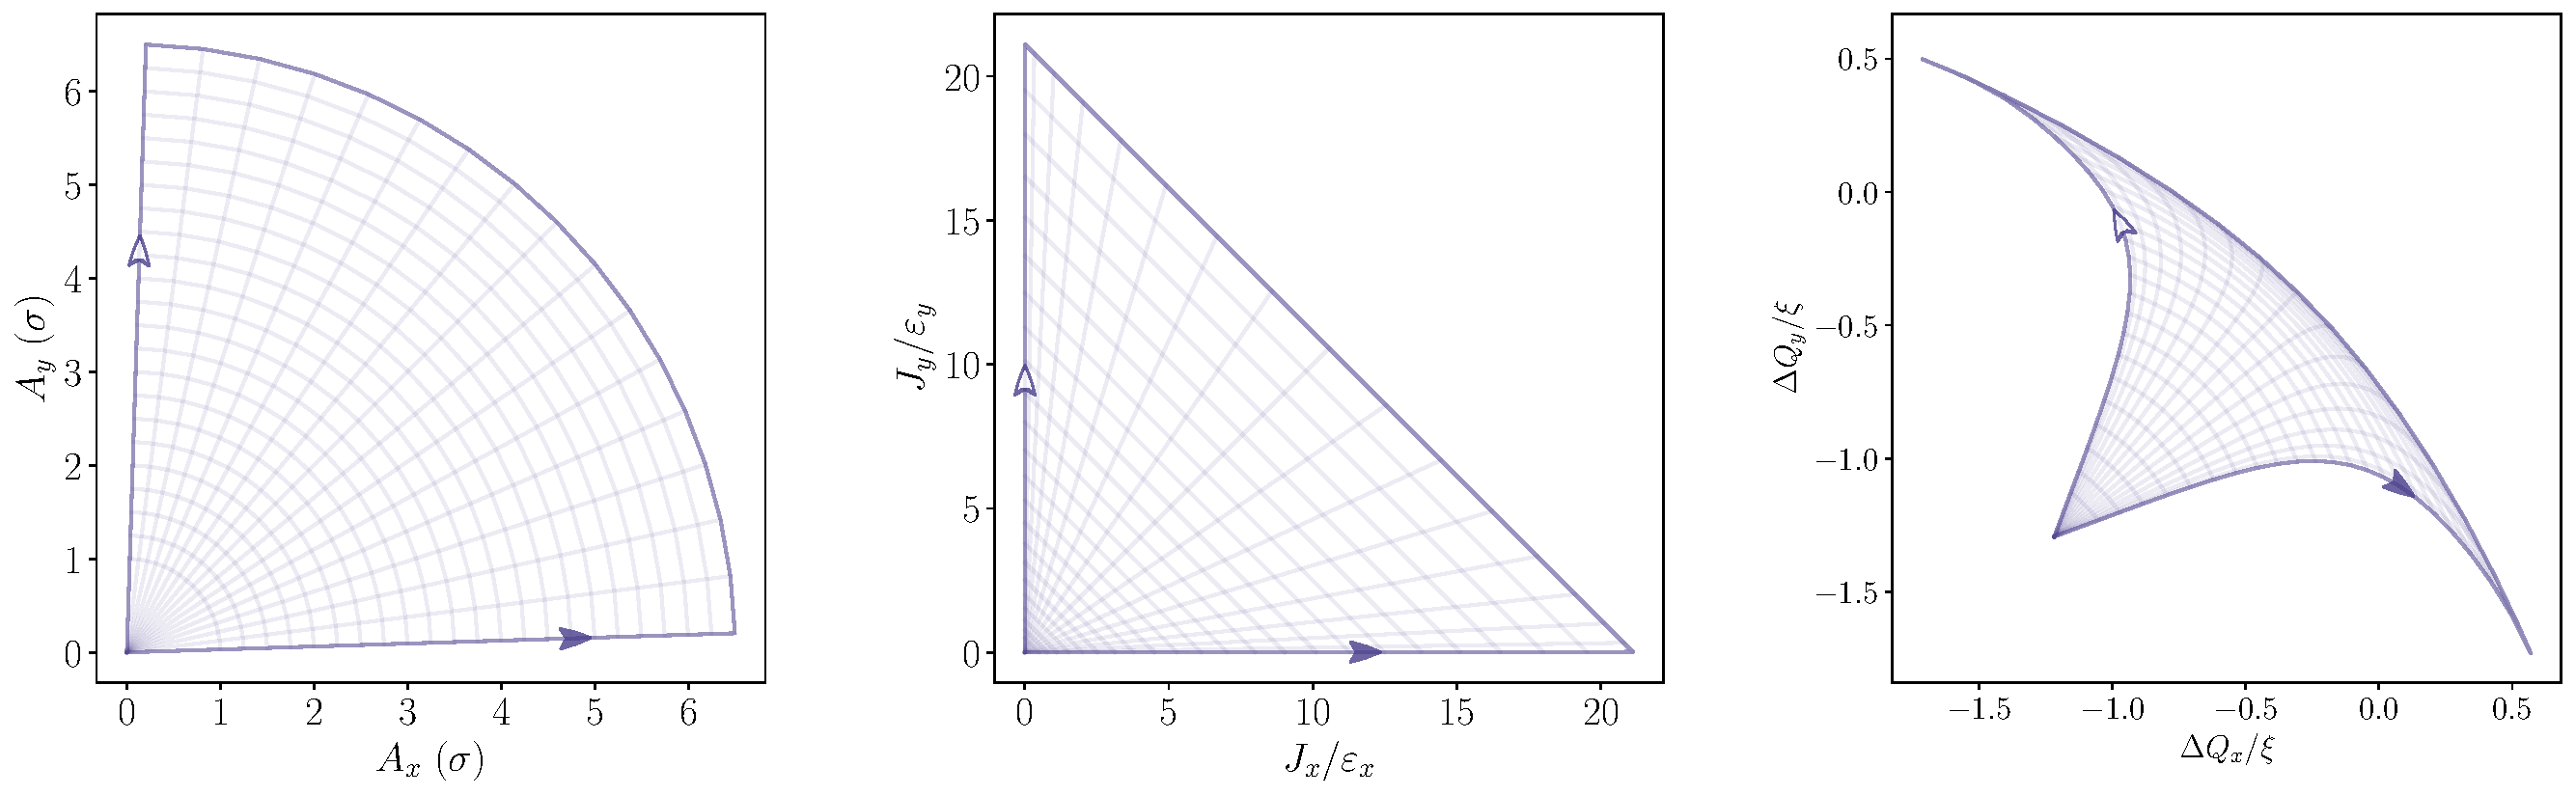
\includegraphics[width=\linewidth]{TeX/Figures/Mapping_explained.pdf}
    \caption{Caption}
    \label{fig:my_label}
\end{figure}


\begin{figure}[h!]
    \centering
    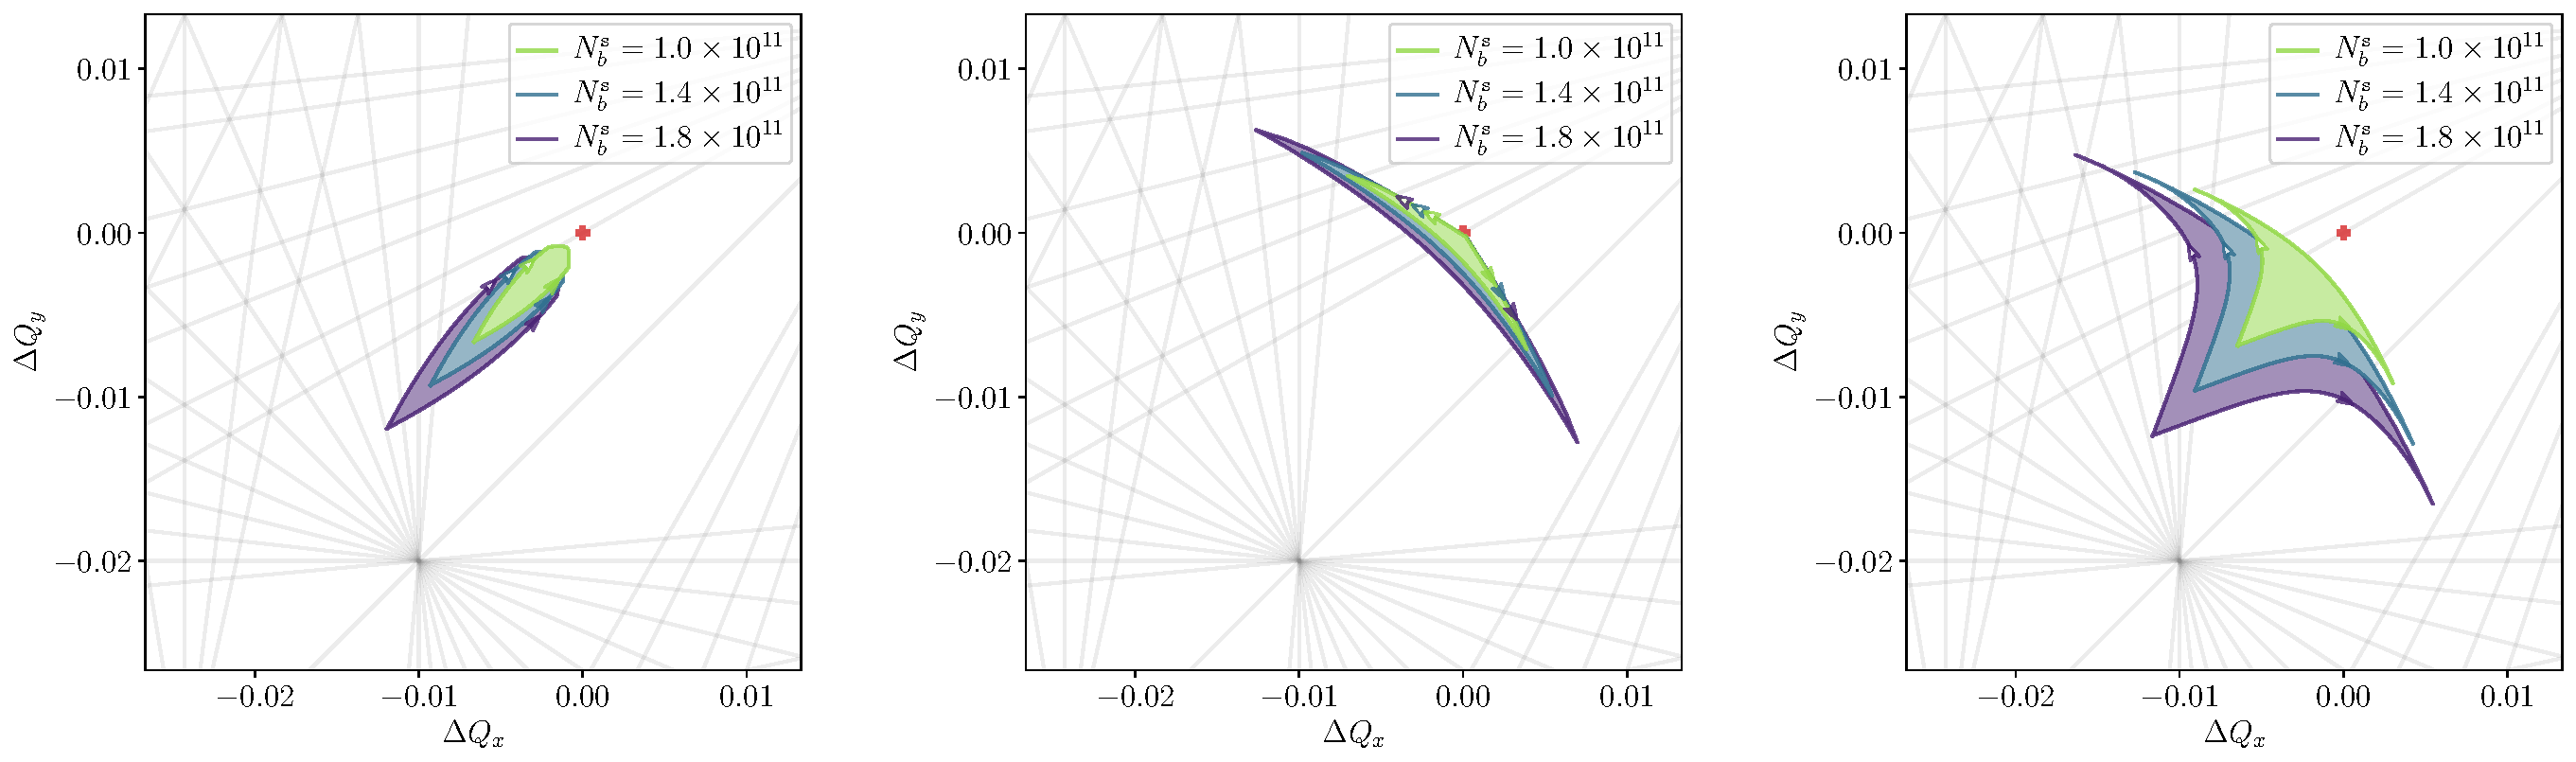
\includegraphics[width=\linewidth]{TeX/Figures/Nb_cmp.pdf}
    \caption{Caption}
    \label{fig:my_label}
\end{figure}

\begin{figure}[h!]
    \centering
    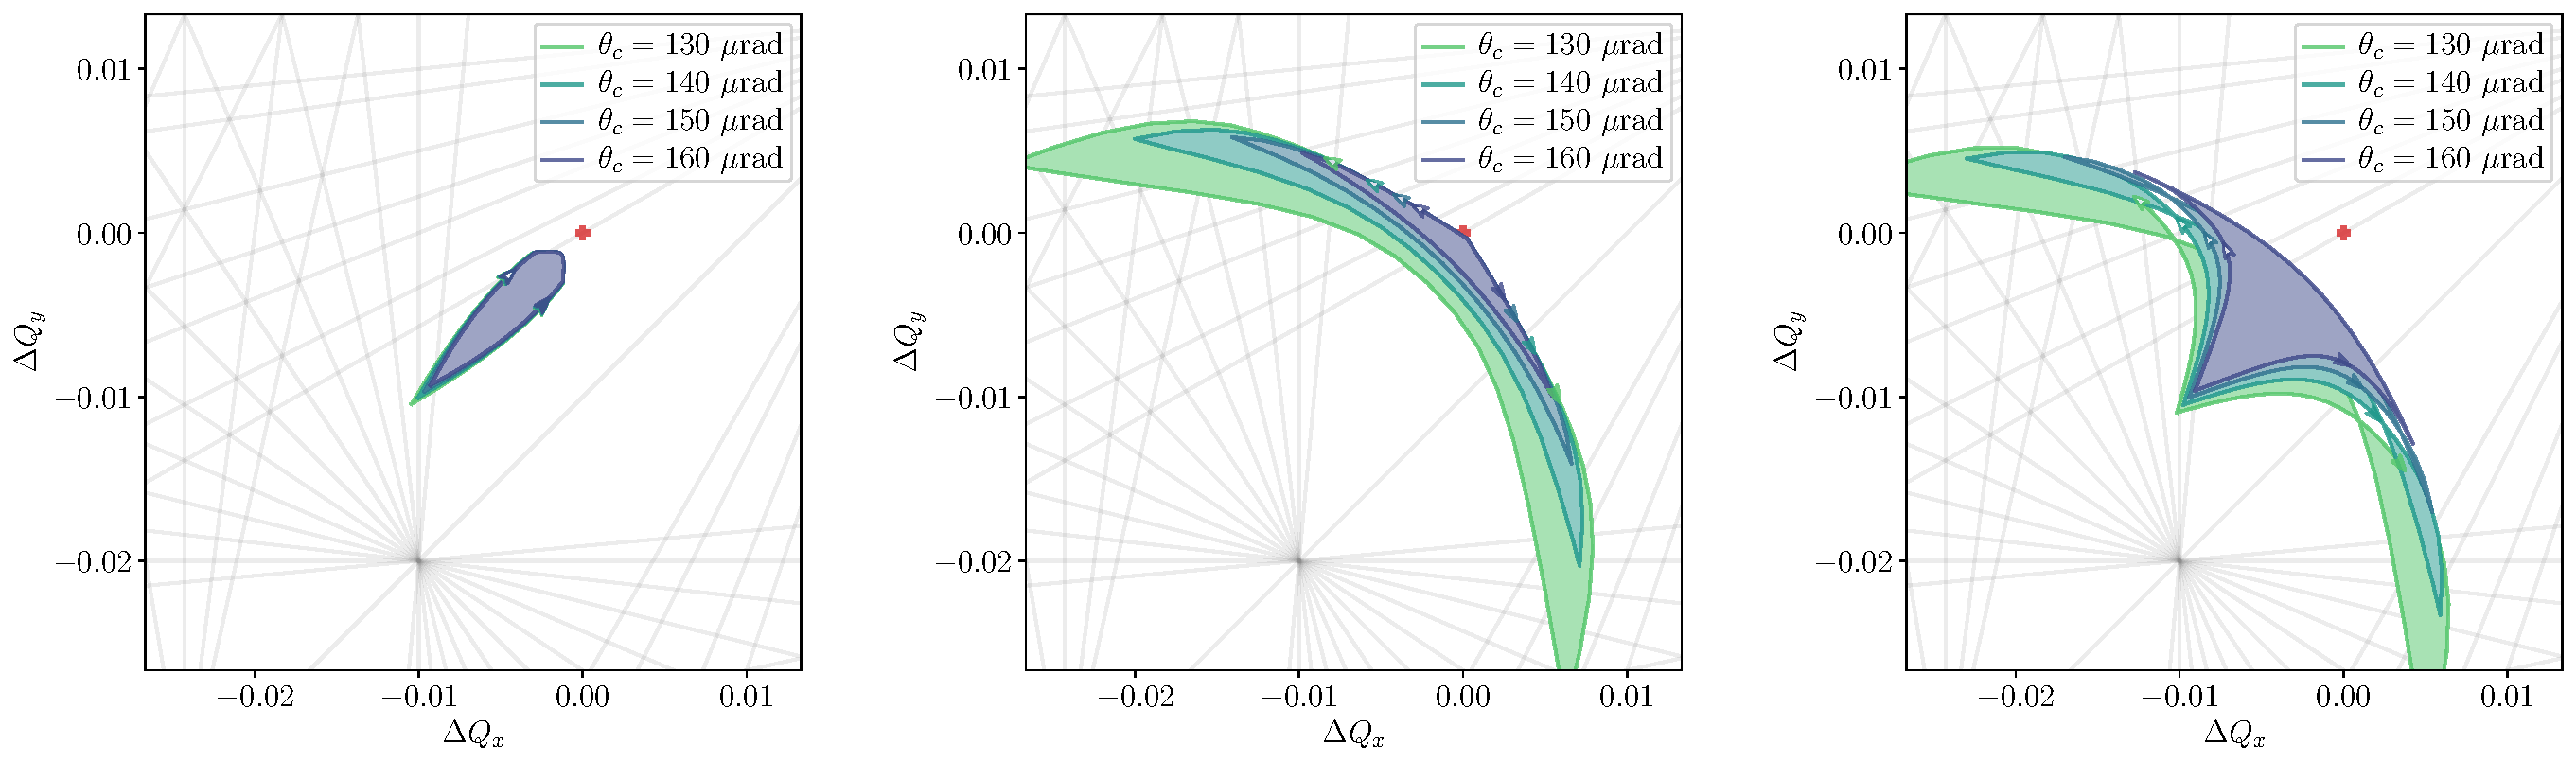
\includegraphics[width=\linewidth]{TeX/Figures/xing_cmp.pdf}
    \caption{Caption}
    \label{fig:my_label}
\end{figure}



\section{Conclusion}



%\bibliography{references}
%\bibliographystyle{ieeetr}

\end{document}